\documentclass[../../deliverable-two.tex]{subfiles}
\graphicspath{
  {\subfix{../../../screens/}}
}

\begin{document}

\subsection{Aplikacja kliencka}

\begin{figure}[h!]
  \centering\includegraphics[width=\screenswidth]{client/Login.png}
  \caption{Ekran logowania}
\end{figure}

\begin{figure}[h!]
  \centering\includegraphics[width=\screenswidth]{client/Main screen.png}
  \caption{Główny widok zawierający dostępność maszyn}
\end{figure}

\subsection{Panel administratora}

Panel administratora posiada skromny interfejs umożliwiający zalogowanie się oraz podgląd zużycia zasobów.

\begin{figure}[h!]
  \centering\includegraphics[width=\screenswidth]{admin/Login.png}
  \caption{Ekran logowania}
\end{figure}

\begin{figure}[h!]
  \centering\includegraphics[width=\screenswidth]{admin/Main screen.png}
  \caption{Widok zużycia zasobów}
\end{figure}

Na tym widoku możemy zobaczyć zużycie zasobów globalne oraz dla każdego z serwerów wirtualizacji. Dodatkowo dla serwera wyświetlona jest również ilość działających i możliwych do uruchomienia maszyn każdego z typów.

\end{document}